\documentclass{article}
\usepackage[utf8]{inputenc}
\usepackage[a4paper,top=2cm,bottom=2cm,left=3cm,right=3cm,marginparwidth=1.75cm]{geometry}
\usepackage{amsmath}
\usepackage{graphicx}
\usepackage{subfig}
\usepackage[colorlinks=true, allcolors=blue]{hyperref}

\begin{document}

\begin{titlepage}

\center % Center everything on the page

\newcommand{\HRule}{\rule{\linewidth}{0.4mm}} % Barra horizontal

\begin{figure}[h!]
    \centering
    
\includegraphics[width=0.24\linewidth]{images/uniMinho.jpg}
\end{figure}

%\textsc{\Large Universidade do Minho}\\[0.75cm]  % Name of your university/college
\textsc{\Large Licenciatura em Ciências da Computação}\\[0.4cm] % Nome do curso
\textsc{\Large Sistemas de Comunicações e Redes}\\[5cm]

{\Large\bfseries Ensaio Escrito}\\[0.5cm]
{\LARGE \bfseries Aplicações e Camada de Transporte} % Título


\vspace{5cm} % Autores
{\bfseries Grupo 28} \\ \vspace{3mm}
Davide Santos (A102938) \\ \vspace{3mm}
Edgar Araújo (A102946) \\ \vspace{3mm}
Pedro Augusto Camargo (A102504) \\ \vspace{3mm}
\vspace{0.2cm}
{Dezembro 2023}\\[0.2cm] % Data

\vfill % Fill the rest of the page with whitespace
\end{titlepage}

\tableofcontents
\pagebreak

\section{Nível aplicacional}
\subsection{Identifique o endereço IP da estação que formulou a query DNS e o tipo de query realizada.}
\begin{figure}[h!]
    \centering
    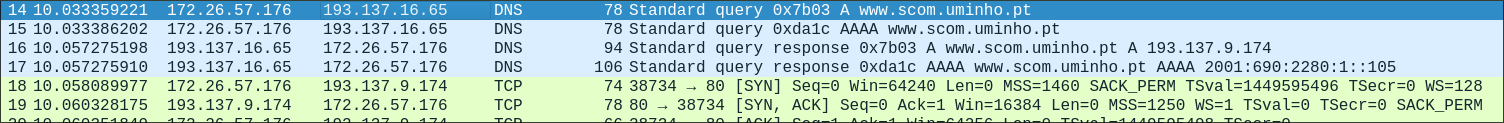
\includegraphics[width=1\linewidth]{images/dns.png}
\end{figure}

O endereço IP da estação que formulou a query DNS: 172.26.57.176 (O meu computador)
Foram enviadas 2 querys dns, uma do tipo A (endereço IPv4) e outra do tipo AAAA (endereço IPv6)

\subsection{Localize a trama com a resposta à query DNS formulada. Identifique nesta trama o endereço IP do
servidor web. Identifique também o servidor de nomes que forneceu a resposta, através do seu IP e nome}

\begin{figure}[h!]
    \centering
    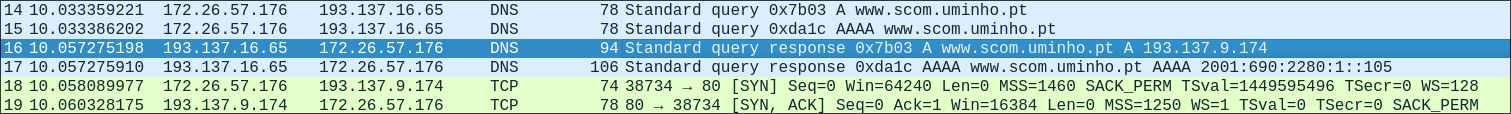
\includegraphics[width=1\linewidth]{images/dns_response.png}
\end{figure}

O endereço IP do servidor web que respondeu a query DNS: 193.137.16.65
De forma a identificar o servidor de nomes que forneceu a resposta, poderia ter sido usado o utilitario nslookup, como tambem o servico WEB https://whatismyipaddress.com/ip/\textless ip\textgreater,
para o ip anterior:
\begin{figure}[h!]
    \centering
    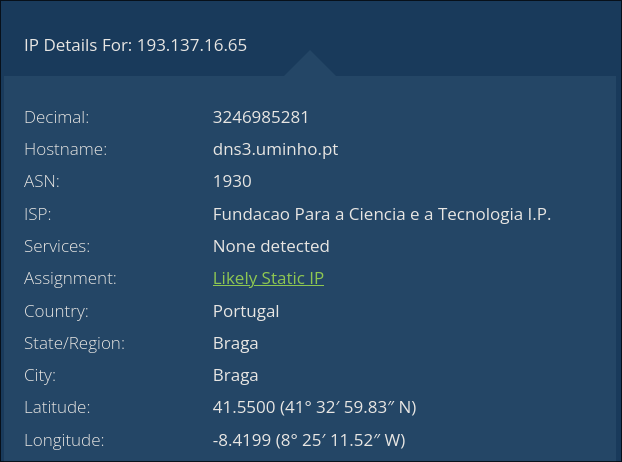
\includegraphics[width=0.5\linewidth]{images/whats.png}
\end{figure}

Obtemos que o servidor DNS que forneceu a resposta, tem por hostname: dns3.uminho.pt

\subsection{Aplique o filtro aos protocolos http // tcp. Identifique os endereços IP do cliente e do servidor HTTP}
\begin{figure}[h!]
    \centering
    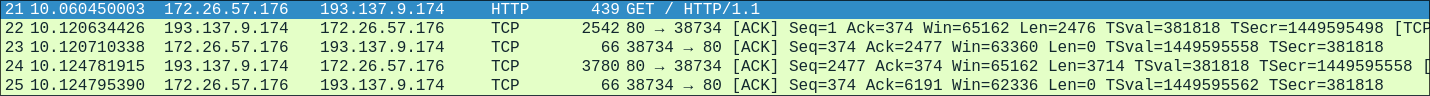
\includegraphics[width=1\linewidth]{images/http_ip.png}
\end{figure}

\begin{itemize}
    \item Temos o endereco IP do cliente, vindo do HTTP GET Request: 172.26.57.176
    \item Que tem como destino o IP do servidor: 193.137.9.174
\end{itemize}

\subsection{Identifique os segmentos TCP correspondentes ao estabelecimento da ligação entre o cliente e o servidor
HTTP. Qual o o tamanho máximo de segmento (MSS) que o servidor aceita receber?}

\begin{figure}[h!]
    \centering
    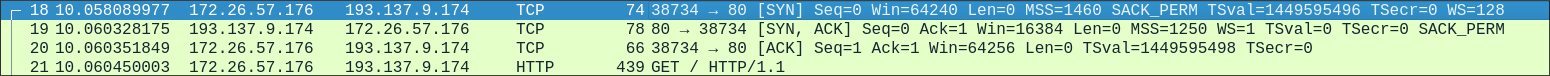
\includegraphics[width=1\linewidth]{images/mss.png}
\end{figure}

Tal como mostra a imagem, os pacotes 18 e 19 correspondem aos pactoes SYN do cliente e SYN-ACK do servidor, respetivamente.
Logo ambos tem oportunidade nestes pacotes de solicitar um MSS, que no caso do servidor é de 1250 bytes.

\subsection{Identifique a resposta HTTP do servidor respeitante ao primeiro pedido GET efetuado pelo cliente.
Quantos bytes de dados aplicacionais contém essa resposta HTTP?}

\begin{figure}[h!]
    \centering
    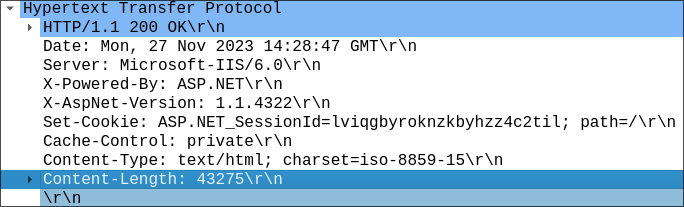
\includegraphics[width=0.5\linewidth]{images/ok.png}
\end{figure}

A resposta HTTP do servidor é do tipo 200 OK, e contem 43275 bytes de dados aplicacionais, tal como indica o campo Content-Length.

\subsection{A resposta HTTP identificada na alínea anterior foi transmitida em quantos segmentos TCP? Apresente
também uma estimativa teórica para essa quantidade.}

\begin{figure}[h!]
    \centering
    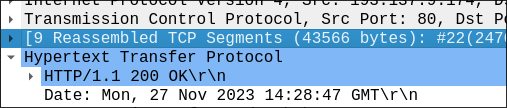
\includegraphics[width=0.5\linewidth]{images/segments.png}
\end{figure}

A resposta HTTP foi transmitida em 9 segmentos. A estimativa teórica para essa quantidade é de 43566/1460 = 29.8, ou seja, 30 segmentos.

\subsection{A partir da informação contida nos cabeçalhos dos protocolos IP e TCP, determine o número de bytes de
dados enviados no primeiro e no último segmento TCP respeitantes à resposta HTTP.}

\begin{figure}[h!]
    \centering
    \subfloat[\centering Primeiro Segmento]{{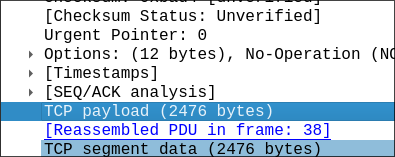
\includegraphics[width=5cm]{images/start.png} }}
    \qquad
    \subfloat[\centering Último Segmento]{{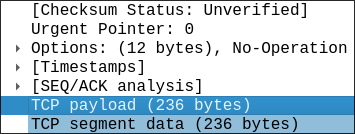
\includegraphics[width=5cm]{images/end.png} }}
\end{figure}

No primeiro segmento TCP, o número de bytes de dados enviados é de 2476 bytes. No último segmento TCP, o número de bytes de dados enviados é de 236 bytes.

\subsection{Observe a informação apresentada no campo host do cabeçalho do pedido HTTP e diga qual o seu
interesse?}

\begin{figure}[h!]
    \centering
    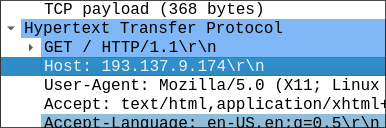
\includegraphics[width=0.5\linewidth]{images/host.png}
\end{figure}

O campo host do cabeçalho do pedido HTTP indica o nome colocado no url do browser, que serve para identificar o website que se pretende aceder, em caso de um servidor conter vários websites diferentes.

\subsection{Com base na sequência de dados trocados entre o cliente e o servidor diga, justificando, se o servidor
HTTP está a funcionar em modo de conexão persistente ou não persistente.}

\begin{figure}[h!]
    \centering
    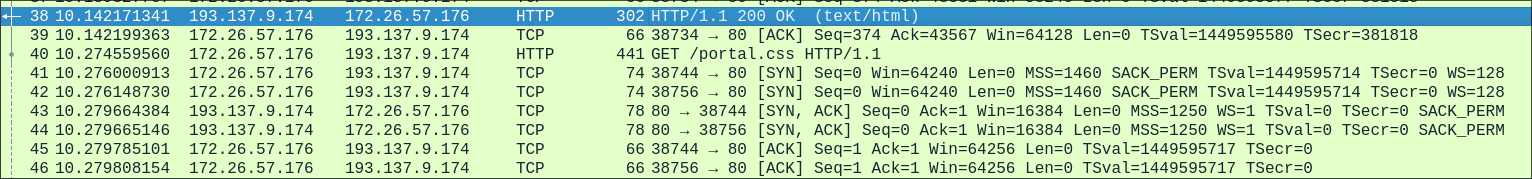
\includegraphics[width=1\linewidth]{images/conexao.png}
\end{figure}

O servidor HTTP está a funcionar em modo de conexão persistente, pois nenhum dos segmentos TCP tem a flag FIN ativa, entre GET Requests.

\subsection{Aceda a https://www.uminho.pt, ao mesmo tempo que captura o tráfego desse acesso com o Wireshark.
Porque razão o tráfego HTTP não é identificado como tal no Wireshark? Apesar disso, pode detetar-se
qual o protocolo aplicacional. Como é que o Wireshark sabe que se trata duma ligação http-over-tls?}

A razao pela qual o trafego HTTP nao é identificado como tal no Wireshark, é porque o trafego HTTP está a ser feito sobre o protocolo TLS, que é um protocolo de segurança que encripta o trafego HTTP, de forma a que este não seja visivel a terceiros. O Wireshark sabe que se trata de uma ligação http-over-tls, porque o protocolo TLS é identificado no campo Protocol do pacote.

\subsection{Diga, justificando, quais dos seguintes elementos uma comunicação HTTPS permite manter ocultos dum
atacante: i) o endereço IP do cliente, ii) o endereço IP do servidor web, iii) o nome do servidor web, iv) o
tamanho da mensagem trocada entre o cliente o servidor, v) a identificação da página acedida no servidor
web, vi) a frequência das conexões estabelecidas entre o cliente e o servidor, vii) os dados da aplicação
trocados entre o servidor e o cliente}

\begin{itemize}
    \item i) O endereço IP do cliente não é oculto, pois é necessário para que o servidor saiba para onde enviar a resposta.
    \item ii) O endereço IP do servidor web não é oculto, pois é necessário para que o cliente saiba para onde enviar o pedido.
    \item iii) O nome do servidor web não é oculto, pois é necessário para que o servidor saiba para que website enviar o pedido.
    \item iv) O tamanho da mensagem trocada entre o cliente e o servidor não é oculto, pois é necessário para que o cliente saiba se recebeu a mensagem completa.
    \item v) A identificação da página acedida no servidor web não é oculto. O caminho do URL é parte da solicitação HTTP e, embora a comunicação seja criptografada, a estrutura básica da solicitação permanece visível.
    \item vi) A frequência das conexões estabelecidas entre o cliente e o servidor não é oculto, pois é necessário para que o servidor saiba se o cliente está a tentar fazer um ataque de negação de serviço.
    \item vii) Os dados da aplicação trocados entre o servidor e o cliente SÃO ocultos, isso garante que o conteúdo da mensagem, incluindo informações sensíveis, não seja visível para um atacante que possa interceptar a comunicação. 
\end{itemize}

\section{Consultas ao serviço de resolução de nomes DNS}

\subsection{Usando os registos do tipo A, identifique os endereços IPv4 dos servidores mail.uminho.pt e
www.ualg.pt? Qual o servidor de nomes que a sua máquina está a usar?}

\begin{figure}[h!]
    \centering
    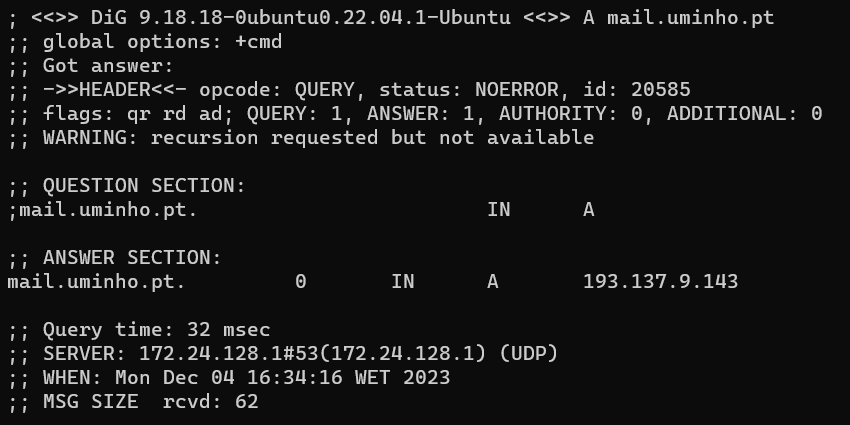
\includegraphics[width=1\textwidth]{images/ex1.mail.png}
    \caption{\label{fig:comando}Output do comando \textit{dig A mail.uminho.pt}}
\end{figure}

\begin{figure} [h!]
    \centering
    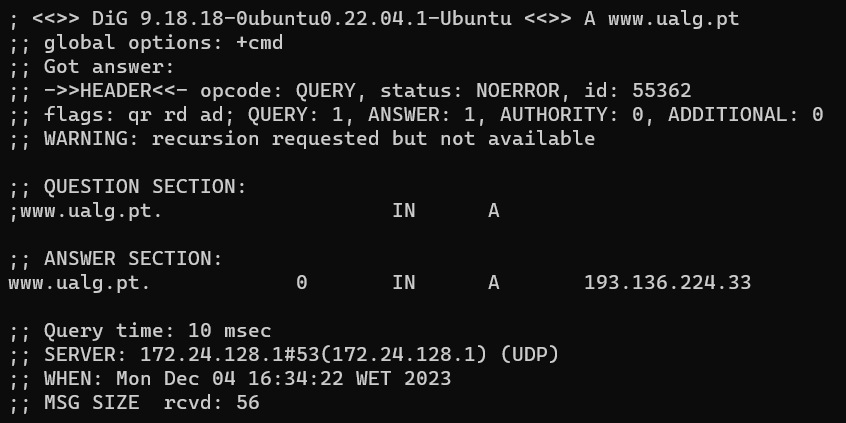
\includegraphics[width=1\textwidth]{images/ex1.ualg.png}
    \caption{\label{fig:comando1}Output do comando \textit{dig A www.ualg.pt}}
\end{figure}

\begin{figure} [h!]
    \centering
    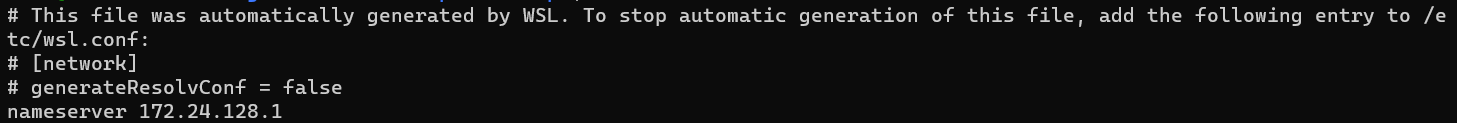
\includegraphics[width=1\textwidth]{images/ex1.resolv.png}
    \caption{\label{fig:comando2}Output do comando \textit{cat /etc/resolv.conf}}
\end{figure}


\begin{itemize}
    \item O endereço IPv4 do servidor \textit{mail.uminho.pt} é \textit{193.137.9.143}.
    \item O endereço IPv4 do servidor \textit{www.ualg.pt} é \textit{193.136.224.33}.
    \item O servidor de nomes utilizado pela sua máquina é \textit{172.24.128.1}.
\end{itemize}

O servidor de nomes utilizado pela máquina é, na verdade, uma \textit{bridge} para a 
minha máquina principal, uma vez que estou a usar wsl2. O servidor de nomes utilizado 
pela máquina principal é: 
\textit{193.137.16.65}, \textit{193.137.16.145} e \textit{193.137.16.75}

\begin{figure} [h!]
    \centering
    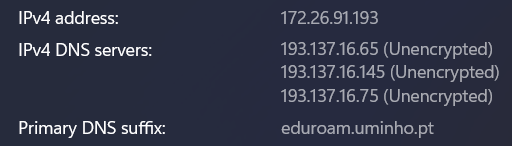
\includegraphics[width=1\textwidth]{images/ex1.windows.png}
    \caption{\label{fig:windows}IPv4 DNS do servidor de nomes da máquina principal}
\end{figure}

\subsection{Usando os registos do tipo PTR, efetue uma query para 
143.9.137.193.in-addr.arpa. O que permitiu identificar esta query?}

\begin{figure} [h!]
    \centering
    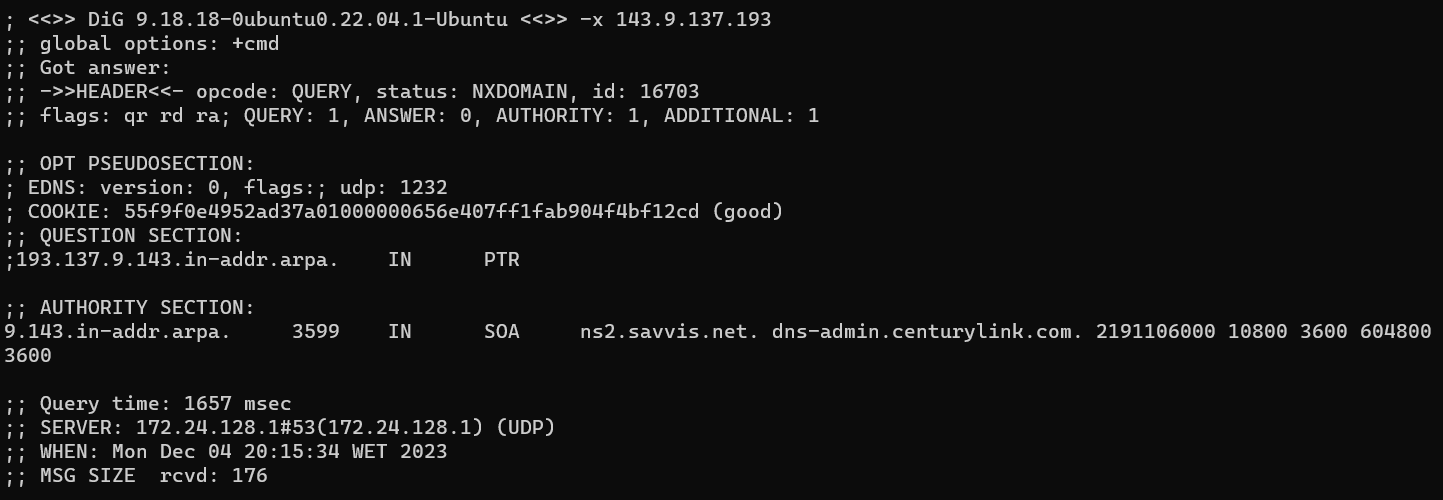
\includegraphics[width=1\textwidth]{images/ex2.143arpa.png}
    \caption{\label{fig:comando3}}Output do comando \textit{dig -x 143.9.137.193}
\end{figure}


A consulta PTR para \texttt{143.9.137.193.in-addr.arpa} resultou em 
um status de \texttt{NXDOMAIN} (não encontrado), indicando que não há 
um registro PTR associado a esse endereço IP. A resposta também 
inclui informações sobre a autoridade, mostrando que o domínio 
\texttt{9.143.in-addr.arpa} tem um registro SOA associado.


\subsection{Certas aplicações fazem uso do reverse DNS, como, por exemplo, o traceroute. Experimente fazer
traceroute (tracert no Windows) para router-di.uminho.pt, ao mesmo tempo que captura o tráfego gerado
com o Wireshark. Comente a diferença observada, em termos de tráfego DNS gerado, entre usar a opção
com e sem resolução de nomes (-n no Linux, -d no Windows). Perante o observado, diga qual a utilidade
que o reverse DNS oferece ao traceroute?}

\begin{figure} [h!]
    \centering
    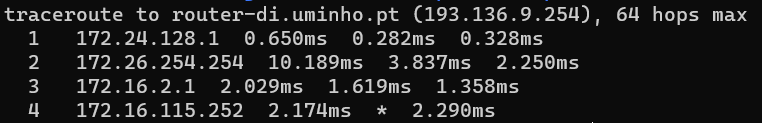
\includegraphics[width=1\textwidth]{images/ex3.traceroute.png}
    \caption{\label{fig:comando4}}Output do comando \textit{traceroute router-di.uminho.pt}
\end{figure}

O comando \texttt{traceroute} foi executado para o destino 
\texttt{router-di.uminho.pt} com o endereço IP \texttt{193.136.9.254}. 
Os resultados mostram o tempo de resposta (em milissegundos) para cada 
salto no caminho até o destino. No quarto salto, houve uma perda de 
pacotes indicada pelo asterisco (*).

\begin{enumerate}
    \item \textbf{Primeiro Salto (172.24.128.1):}
        \begin{itemize}
            \item Tempo de resposta: 0.650ms, 0.282ms, 0.328ms.
        \end{itemize}
    
    \item \textbf{Segundo Salto (172.26.254.254):}
        \begin{itemize}
            \item Tempo de resposta: 10.189ms, 3.837ms, 2.250ms.
        \end{itemize}
    
    \item \textbf{Terceiro Salto (172.16.2.1):}
        \begin{itemize}
            \item Tempo de resposta: 2.029ms, 1.619ms, 1.358ms.
        \end{itemize}
    
    \item \textbf{Quarto Salto (172.16.115.252):}
        \begin{itemize}
            \item Tempo de resposta: 2.174ms, * (perda de pacotes), 2.290ms.
        \end{itemize}
  \end{enumerate}
  
  A perda de pacotes no quarto salto pode indicar uma interrupção 
  temporária na comunicação ou congestionamento na rede nesse ponto 
  específico. O aumento no tempo de resposta nos saltos subsequentes 
  pode ser causado por várias razões, como a distância física, 
  congestão de rede ou configuração específica dos \textit{routers}.
  

\subsection{Usando o registo NS:}

\begin{itemize}
    \item Para o domínio "tecnico.ulisboa.pt." (tamanho do pacote de resposta: 381 bytes):


    \begin{verbatim}
tecnico.ulisboa.pt.     0       IN      NS      ns2.tecnico.ulisboa.pt.
tecnico.ulisboa.pt.     0       IN      NS      a.ul.pt.
tecnico.ulisboa.pt.     0       IN      NS      ns1.tecnico.ulisboa.pt.
a.ul.pt.                0       IN      A       194.117.0.150
ns1.tecnico.ulisboa.pt. 0       IN      A       193.136.128.1
ns2.tecnico.ulisboa.pt. 0       IN      A       193.136.128.2
a.ul.pt.                0       IN      AAAA    2001:690:21c0:a::150
ns1.tecnico.ulisboa.pt. 0       IN      AAAA    2001:690:2100:1::53:1
ns2.tecnico.ulisboa.pt. 0       IN      AAAA    2001:690:2100:1::2
\end{verbatim}

    \item Para o domínio "ulisboa.pt." (tamanho do pacote de resposta: 444 bytes):


    \begin{verbatim}
ulisboa.pt.             0       IN      NS      ns1.tecnico.ulisboa.pt.
ulisboa.pt.             0       IN      NS      ns2.tecnico.ulisboa.pt.
ulisboa.pt.             0       IN      NS      a.ul.pt.
ulisboa.pt.             0       IN      NS      b.ul.pt.
a.ul.pt.                0       IN      A       194.117.0.150
b.ul.pt.                0       IN      A       194.117.1.150
ns1.tecnico.ulisboa.pt. 0       IN      A       193.136.128.1
ns2.tecnico.ulisboa.pt. 0       IN      A       193.136.128.2
a.ul.pt.                0       IN      AAAA    2001:690:21c0:a::150
b.ul.pt.                0       IN      AAAA    2001:690:21c0:b::150
ns1.tecnico.ulisboa.pt. 0       IN      AAAA    2001:690:2100:1::53:1
ns2.tecnico.ulisboa.pt. 0       IN      AAAA    2001:690:2100:1::2
\end{verbatim}

    \item Para o domínio "pt." (tamanho do pacote de resposta: 658 bytes):


    \begin{verbatim}
pt.                     0       IN      NS      d.dns.pt.
pt.                     0       IN      NS      ns.dns.br.
pt.                     0       IN      NS      e.dns.pt.
pt.                     0       IN      NS      a.dns.pt.
pt.                     0       IN      NS      ns2.nic.fr.
pt.                     0       IN      NS      b.dns.pt.
pt.                     0       IN      NS      h.dns.pt.
pt.                     0       IN      NS      g.dns.pt.
pt.                     0       IN      NS      c.dns.pt.
a.dns.pt.               0       IN      A       185.39.208.1
b.dns.pt.               0       IN      A       194.0.25.23
c.dns.pt.               0       IN      A       204.61.216.105
d.dns.pt.               0       IN      A       185.39.210.1
e.dns.pt.               0       IN      A       193.136.192.64
g.dns.pt.               0       IN      A       193.136.2.226
h.dns.pt.               0       IN      A       194.146.106.138
ns.dns.br.              0       IN      A       200.160.0.5
ns2.nic.fr.             0       IN      A       192.93.0.4
a.dns.pt.               0       IN      AAAA    2a04:6d80::1
b.dns.pt.               0       IN      AAAA    2001:678:20::23
c.dns.pt.               0       IN      AAAA    2001:500:14:6105:ad::1
d.dns.pt.               0       IN      AAAA    2a04:6d82::1
e.dns.pt.               0       IN      AAAA    2001:690:a00:4001::64
g.dns.pt.               0       IN      AAAA    2001:690:a80:4001::100
\end{verbatim}

    \item Para o domínio "." (tamanho do pacote de resposta: 966 bytes):


    \begin{verbatim}
.                       0       IN      NS      e.root-servers.net.
.                       0       IN      NS      d.root-servers.net.
.                       0       IN      NS      a.root-servers.net.
.                       0       IN      NS      l.root-servers.net.
.                       0       IN      NS      g.root-servers.net.
.                       0       IN      NS      b.root-servers.net.
.                       0       IN      NS      h.root-servers.net.
.                       0       IN      NS      j.root-servers.net.
.                       0       IN      NS      f.root-servers.net.
.                       0       IN      NS      i.root-servers.net.
.                       0       IN      NS      m.root-servers.net.
.                       0       IN      NS      c.root-servers.net.
.                       0       IN      NS      k.root-servers.net.
a.root-servers.net.     0       IN      A       198.41.0.4
b.root-servers.net.     0       IN      A       170.247.170.2
c.root-servers.net.     0       IN      A       192.33.4.12
d.root-servers.net.     0       IN      A       199.7.91.13
e.root-servers.net.     0       IN      A       192.203.230.10
f.root-servers.net.     0       IN      A       192.5.5.241
g.root-servers.net.     0       IN      A       192.112.36.4
h.root-servers.net.     0       IN      A       198.97.190.53
i.root-servers.net.     0       IN      A       192.36.148.17
j.root-servers.net.     0       IN      A       192.58.128.30
k.root-servers.net.     0       IN      A       193.0.14.129
l.root-servers.net.     0       IN      A       199.7.83.42
m.root-servers.net.     0       IN      A       202.12.27.33
a.root-servers.net.     0       IN      AAAA    2001:503:ba3e::2:30
b.root-servers.net.     0       IN      AAAA    2801:1b8:10::b
\end{verbatim}

\end{itemize}


\subsubsection{Identifique os servidores de nomes definidos para os 
domínios: “tecnico.ulisboa.pt.”, “ulisboa.pt.”, “pt.” e “.” (root).}

\begin{enumerate}
    \item \textbf{tecnico.ulisboa.pt.:}
        \begin{itemize}
            \item ns2.tecnico.ulisboa.pt.
            \item a.ul.pt.
            \item ns1.tecnico.ulisboa.pt.
        \end{itemize}
    \item \textbf{ulisboa.pt.:}
        \begin{itemize}
            \item ns1.tecnico.ulisboa.pt.
            \item ns2.tecnico.ulisboa.pt.
            \item a.ul.pt.
            \item b.ul.pt.
        \end{itemize}
    \item \textbf{pt.:}
        \begin{itemize}
            \item d.dns.pt.
            \item ns.dns.br.
            \item e.dns.pt.
            \item a.dns.pt.
            \item ns2.nic.fr.
            \item b.dns.pt.
            \item h.dns.pt.
            \item g.dns.pt.
            \item c.dns.pt.
        \end{itemize}
    \item \textbf{. (root):}
        \begin{itemize}
            \item e.root-servers.net.
            \item d.root-servers.net.
            \item a.root-servers.net.
            \item l.root-servers.net.
            \item g.root-servers.net.
            \item b.root-servers.net.
            \item h.root-servers.net.
            \item j.root-servers.net.
            \item f.root-servers.net.
            \item i.root-servers.net.
            \item m.root-servers.net.
            \item c.root-servers.net.
            \item k.root-servers.net.
        \end{itemize}
\end{enumerate}


\subsubsection{Perante a informação obtida, diga, justificando, se os servidores de nomes de diferentes domínios
podem coexistir numa mesma máquina física.}

Os resultados indicam que os servidores de nomes para diferentes 
domínios estão hospedados em máquinas distintas. No entanto, apenas 
com os registros NS, não podemos afirmar conclusivamente se estão em 
máquinas físicas separadas. Para uma conclusão mais precisa, seria 
necessário verificar informações adicionais, como endereços IP e 
configurações específicas.


\subsubsection{Encontra domínios geridos por servidores de nomes localizados em redes IP distintas? Se sim,
apresente esses domínios e diga qual a vantagem resultante desse procedimento?}

Sim, é possível identificar domínios geridos por servidores de nomes 
localizados em redes IP distintas. Por exemplo, ao observar os 
servidores de nomes para o domínio "pt.", notamos que eles estão 
distribuídos em várias redes IP. Isso é uma prática comum para 
garantir redundância e maior robustez na infraestrutura de DNS. 
Alguns desses domínios são:

\begin{itemize}
    \item d.dns.pt
    \item ns.dns.br
    \item e.dns.pt
    \item a.dns.pt
    \item ns2.nic.fr
    \item b.dns.pt
    \item h.dns.pt
    \item g.dns.pt
    \item c.dns.pt
\end{itemize}

A vantagem de ter servidores de nomes em redes IP distintas está na 
resiliência do sistema. Se uma rede ou servidor falhar, outros ainda 
podem responder às consultas DNS, garantindo a disponibilidade 
contínua dos serviços.


\subsection{Usando o registo SOA:}

\subsubsection{Identifique o servidor DNS primário definido para os domínios: “tecnico.ulisboa.pt.”,
“ulisboa.pt.”, “pt.” e “.” (root).}

\begin{enumerate}
    \item \textbf{tecnico.ulisboa.pt.:}
        \begin{itemize}
            \item ns2.tecnico.ulisboa.pt.
        \end{itemize}
    \item \textbf{ulisboa.pt.:}
        \begin{itemize}
            \item ns1.tecnico.ulisboa.pt.
        \end{itemize}
    \item \textbf{pt.:}
    \begin{itemize}
        \item d.dns.pt.
    \end{itemize}
    \item \textbf{. (root):}
    \begin{itemize}
        \item a.root-servers.net.
    \end{itemize}
\end{enumerate}

\subsubsection{Quais são os servidores secundários dos domínios “tecnico.ulisboa.pt.” e “ulisboa.pt.”?
Justifique.}

\begin{enumerate}
    \item \textbf{tecnico.ulisboa.pt.:}
        \begin{itemize}
            \item a.ul.pt.
            \item ns1.tecnico.ulisboa.pt.
        \end{itemize}
    \item \textbf{ulisboa.pt.:}
        \begin{itemize}
            \item ns2.tecnico.ulisboa.pt.
        \end{itemize}
\end{enumerate}


Servidores secundários são configurados para armazenar cópias de 
zonas DNS e fornecer redundância e resistência a falhas. No caso:

\begin{itemize}
    \item Para "tecnico.ulisboa.pt.", a.ul.pt. e ns1.tecnico.ulisboa.pt. atuam como servidores secundários.
    \item Para "ulisboa.pt.", ns2.tecnico.ulisboa.pt. é o servidor secundário.
\end{itemize}

\subsubsection{Em que difere o servidor primário de um servidor secundário? Qual o significado dos parâmetros
temporais associados ao servidor primário?}

\textbf{Servidor Primário:}
\begin{itemize}
    \item Contém a cópia principal e autoritativa da zona DNS.
    \item Tem a autoridade final sobre a zona.
    \item Atualizações são feitas diretamente no servidor primário.
\end{itemize}


\textbf{Servidor Secundário:}
\begin{itemize}
    \item Mantém uma cópia secundária (réplica) da zona DNS.
    \item Obtém atualizações do servidor primário periodicamente.
    \item Serve como backup e distribui a carga de consulta.
\end{itemize}

\textbf{Parâmetros temporais associados ao servidor primário:}
\begin{itemize}
    \item \textbf{SOA (Start of Authority):}
        \begin{itemize}
            \item 2191106000: Número de série da zona.
            \begin{itemize}
                \item Incrementa a cada modificação.
            \end{itemize}
            \item 10800: Tempo de espera padrão (3 horas) antes de tentar novamente uma transferência de zona falhada.
            \item 3600: Tempo de espera entre tentativas de transferência de zona.
            \item 604800: Tempo máximo que um servidor secundário espera por uma transferência de zona antes de expirar o registro SOA.
            \item 3600: Tempo de vida padrão para registros negativos (1 hora).
        \end{itemize}
\end{itemize}


\section{Uso da camada de transporte por parte das aplicações}

\subsection{Capturando o tráfego nos momentos que considere adequados, observe atentamente como as várias aplicações
utilizam o serviço de transporte, quando é efetuado}

a) \textbf{browser http://www.sdum.uminho.pt/} - Não é seguro. O protocolo de transporte utilizado é o TCP/IP. Porta 80.

\begin{figure}[h!]
    \centering
    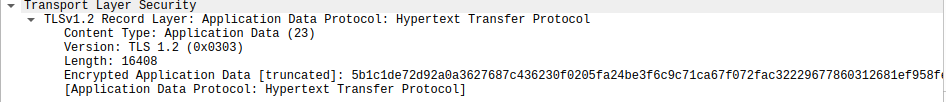
\includegraphics[width=1\textwidth]{images/httpsdata.png}
    \caption{Dados do http nao encriptados}
    \label{fig:enter-label}
\end{figure}

\begin{figure}[h!]
    \centering
    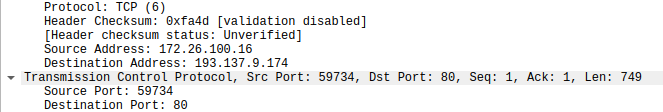
\includegraphics[width=1\textwidth]{images/httpprotocol.png}
    \caption{Porta e protocolo do pedido http}
    \label{fig:enter-label}
\end{figure}



b) \textbf{browser https://www.uminho.pt/PT} - É seguro. Protocolo de Transporte: SSL/TLS. Porta 443.

\begin{figure}[h!]
    \centering
    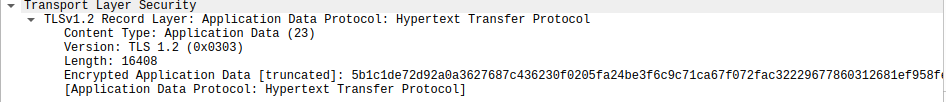
\includegraphics[width=1\textwidth]{images/httpsdata.png}
    \caption{Dados do http encriptados}
    \label{fig:enter-label}
\end{figure}

\begin{figure}[h!]
    \centering
    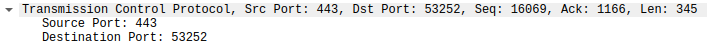
\includegraphics[width=1\textwidth]{images/httpsport.png}
    \caption{Porta do pedido https}
    \label{fig:enter-label}
\end{figure}

\begin{figure}[h!]
    \centering
    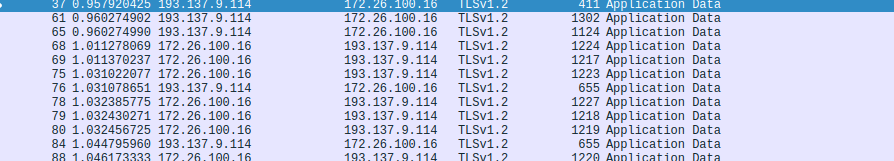
\includegraphics[width=1\textwidth]{images/ssl.png}
    \caption{Protocolo SSL/TLS do pedido https}
    \label{fig:enter-label}
\end{figure}


c) \textbf{ftp ftp.di.uminho.pt} - Não é seguro. Protocolo de transporte: TCP. Portas 20 e 21.

\begin{figure}[h!]
    \centering
    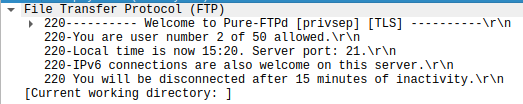
\includegraphics[width=1\textwidth]{images/ftpdados.png}
    \caption{Dados do ftp nao encriptados}
    \label{fig:enter-label}
\end{figure}

\begin{figure}[h!]
    \centering
    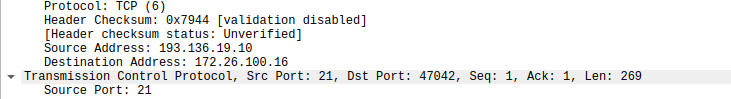
\includegraphics[width=1\textwidth]{images/ftp.png}
    \caption{Porta 21 e Protocolo de Transporte TCP}
    \label{fig:enter-label}
\end{figure}

d) \textbf{ping dns.google} - É seguro. Protocolo de Transporte: ICMP. Não aplicável.

\begin{figure}[h!]
    \centering
    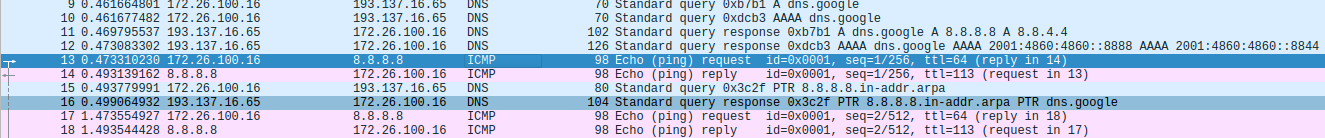
\includegraphics[width=1\textwidth]{images/ping.png}
    \caption{Protocolos ICMP dos pings para 8.8.8.8 (dns.google}
    \label{fig:enter-label}
\end{figure}

e) \textbf{ssh marco.uminho.pt} - É seguro. Protocolo de Transporte: TCP. Porta 22.

\begin{figure}[h!]
    \centering
    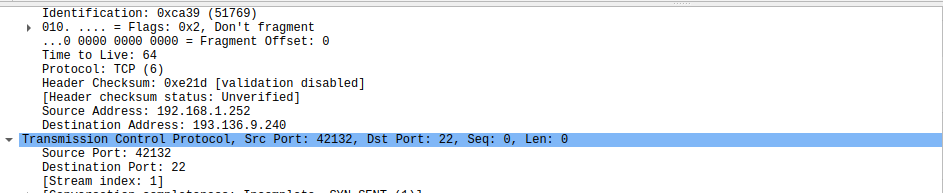
\includegraphics[width=1\textwidth]{images/ssh.png}
    \caption{\label{fig:pacote}Porta e protocolo ssh}
\end{figure}

f) \textbf{nslookup www.ualg.pt} - Não é seguro. Protocolo de Transporte: UDP. Porta 53.

\begin{figure}[h!]
    \centering
    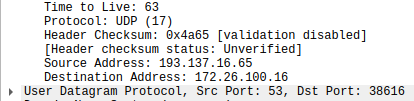
\includegraphics[width=1\textwidth]{images/nslookup.png}
    \caption{\label{fig:pacote}Porta e protocolo nslookup}
\end{figure}

g) \textbf{traceroute dns.uminho.pt} - É seguro. Protocolo de Transporte: UDP e ICMP. Costuma começar na porta 33434 e usa portas com valores altos. 

\begin{figure}[h!]
    \centering
    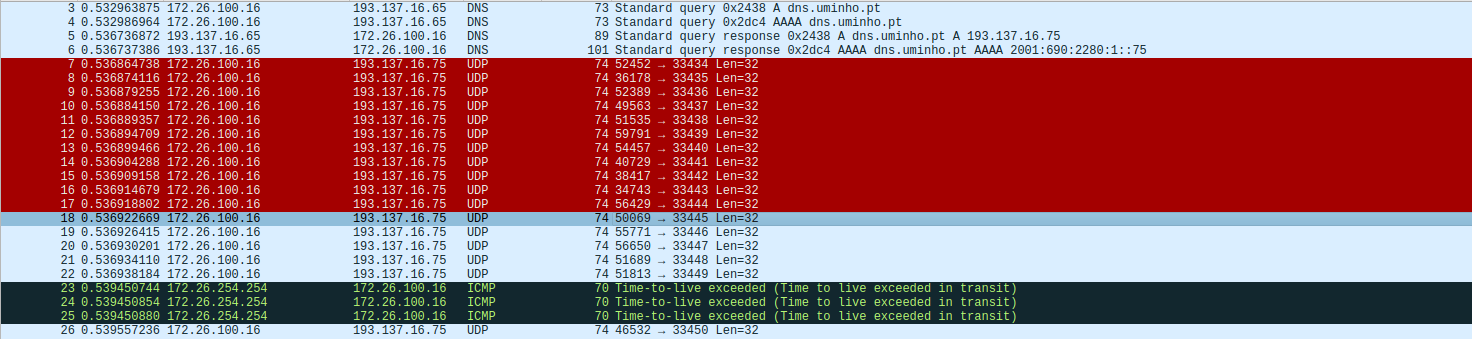
\includegraphics[width=1\textwidth]{images/traceroute.png}
    \caption{\label{fig:pacote}Traceroute}
\end{figure}

h) \textbf{telnet freechess.org} - Não é seguro. Protocolo de Transporte: TCP. Porta 23

\begin{figure}[h!]
    \centering
    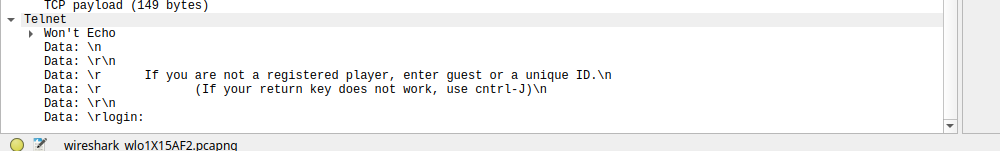
\includegraphics[width=1\textwidth]{images/telnet1.png}
    \caption{Dados não encriptados telnet}
    \label{fig:enter-label}
\end{figure}

\begin{figure}[h!]
    \centering
    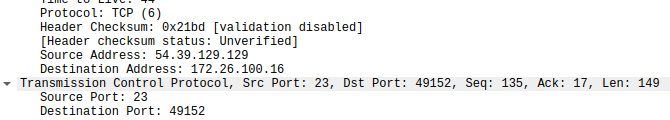
\includegraphics[width=1\textwidth]{images/telnet2.png}
    \caption{Porta e protocolo utilizado telnet}
    \label{fig:enter-label}
\end{figure}

\subsection{Comente as principais diferenças entre os protocolos TCP e UDP. Relacione-as com as experiências realizadas
onde observou os campos dos cabeçalhos respetivos e o overhead protocolar. Em particular, identifique os
campos do TCP responsáveis pelo controlo de fluxo, ordenação e fiabilidade do protocolo. Perante isto, diga,
justificando, se nas aplicações com requisitos temporais críticos (e.g. online gaming, video-audio streaming) é
mais adequado usar o protocolo UDP ou o TCP?}

O \textbf{Protocolo TCP} oferece um serviço mais confiável de entrega de dados, ele retransmite pacotes perdidos no caminho e solicita confirmações de recebimento do destinatário (ACK), já o \textbf{Protocolo UDP} oferece um serviço menos confiável, mas também uma transmissão de dados mais rápida. Como o Protocolo UDP é mais simples comparado com o TCP, resulta em menos overhead. Além disso, o protocolo UDP não requere a confirmação da entrega do pacote e não retransmite pacotes perdidos de forma a corrigir a transmissão. O TCP é garante que os dados sejam entregues na ordem correta ao destinatário, fazendo com que seja mais lento comparado com o UDP. O \textbf{TCP} gere o controlo de fluxo através das Flags TCP, como o flag ACK e a flag Window Update, através do Número de Sequência (Sequence Number), que são utilizados para controlar a ordem dos pacotes e garantir a entrega correta. Quanto à fiabilidade do protocolo, o \textbf{TCP} utiliza um processo de Handshaking para a sincronização e negociação de parâmetros de comunicação.
Nas aplicações com requisitos temporais críticos é mais adequado utilizarmos os protocolo UDP. Em jogos online e streaming, a latência é crítica para uma experiência positiva, por isso, como o Protocolo UDP é o mais rápido, é utilizado nessas ocasiões, além disso, há uma tolerância â perda de pacotes nos jogos e streamings sem a necessidade de retransmissão. O UDP Não espera por ACKs, o que resulta em menor sobrecarga e menor atraso para a entrega de dados.

\section{Conclusao}

Escrever este relatório foi fundamental para entendermos como as comunicações acontecem usando o TCP, um protocolo essencial na transmissão confiável de dados. Exploramos também os protocolos HTTP e HTTP sobre TLS, que são fundamentais para a comunicação com websites, destacando a importância da segurança.

Além disso, aprendemos sobre utilitários como 'dig' e 'nslookup', que são ferramentas práticas para pesquisar em servidores DNS, ajudando a entender como os nomes de domínio são resolvidos.

\end{document}
